\begin{document}
\chapter{Aplicatia MyMusicTeacher}

\section{Definirea problemei}
	Problema tratată de această lucrare de licență o reprezintă proiectarea unei plaftorme de antrenare a rețelelor neuronale convoluționale și o aplicație ce va realiza detectarea vizuală a notelor muzicale pe partitură, în timp real, folosind camera unui dispozitiv mobil. 
	
	Propunem crearea unui sistem inteligent, ce poate fi transpus și poate funcționa la parametri optimi pe o gamă cât mai largă de dispozitive mobile. Acest sistem va primi, în mod continuu, date de intrare de la camera video a dispozivului mobil, va procesa în timp real imaginile, și va aduce o predicție pentru fiecare cadru, reprezentând nota muzicală prezentă pe partitură. 
	
	Dorim sa excludem dependența conexiunii la internet la momentul procesării imaginilor, iar în acest scop propunem crearea unui modul, compatibil cu dispozitive mobile, care să lucreze izolat cu parametrii optimizați de către sistemul inteligent, creat și antrenat pe server, și un serviciu care ruleaza pe o masina cu acces la internet, capabil de a transmite aplicațiilor de pe dispozitivile mobile, parametrii sistemului inteligent. 
	
	Dorim ca sistemul inteligent, prezent pe telefon, să poată fi actualizat cu usurință prin intermediul serviciului.  

\section{Analiza problemei}
	În scopul rezolvării acestei probleme, vom urmari și defini un număr de pași, pentru a modela aplicația și funcționalitățile sale.
	Pentru primul pas în scopul rezolvării acestei probleme, ne vom folosi de ramura învățării automate, specializată în procesarea de imagini. Vom profita de eficiența, la nivel de timp și memorie, oferită de rețelele neuronale convoluționale și vom implementa o aplicație, care permite configurarea si antrenarea unui model.
	
	Aplicația va permite construirea arhitecturii modelului de rețele neuronale convoluționale și alegerea unor parametrii utilizați pe parcursul procesului de învățare, iar pe baza configurației alese va trece modelul prin etapa de antrenare. La finalul  etapei de antrenare, aplicația va crea un fișier de tip JSON, unde va exporta arhitectura modelului împreună cu parametrii acestuia. 
	
	Exportarea fisierului JSON, unde este prezentă o versiune a modelului antrenat, este realizată in scopul plasării acestui model pe un server, responsabil cu departajarea informațiilor tuturor clienților. 
	Pentru antrenarea modelului, vom folosi un set de aproximativ 3500 de imagini, rezultate pe urma augmentării  unui set de imagini realizate cu un dispozitiv mobil și pre-procesate în scopul scoaterii în evidență a informației utile. Pozele vor fi grupate în  7 clase, reprezentând note întregi, simple (fără diez și bemol), de la DO la SI, avănd cca. 500 de imagini per clasa. 
	
	Aplicația va încărca în memorie imaginile, le va procesa pentru a le aduce la dimensiunea optimă antrenării și va gestiona dimensiunile canalelor de imagine, în scopul optimizării complexității de timp al etapei de învățare. După realizarea acestor pasi, aplicația va trece setul de date de intrare printr-o etapă de randomizare, cu scopul înlăturării omogenității, un factor crucial care influențeza capabilitatea modelului de atingere a unei precizii optime, iar pe baza configurației alese aplicația va grupa imaginile și le va transmite modelului în scopul antrenării.
	
	Aplicația va permite monitorizarea, în timp real, a progresului modelului și a preciziei acumulate. La finalul etapei de antrenare, vom exporta într-un fișier progresul antrenării, i.e un istoric, în eventuala posibilitate de a analiza progresul fiecărui model după etapa de antrenare.
	Scopul aplicației va fi: modelarea unei arhitecturi cu o precizie cat mai ridicata.
	Configurările valabile vor fi:
	
	\begin{itemize}
	\item	Alegerea dimensiunii seturilor de antrenare (batch size). Acest parametru va gestiona modul de grupare a imaginilor. În funcție de acest parametru se va calcula dimensiunea setului de date de validare.
	
	
	\item	Construirea arhitecturii prin adăugarea și configurarea straturilor rețelei neuronale convoluționale(layers).  Fiecare strat al rețelei, va fi configurat individual și va fi adăugat în arhitectura modelului. Tipurile de straturi care vor fi prezente în aplicație sunt: Convolution Layer, Max Pooling Layer, Flattening Layer si Hidden Layer. Aceste straturi vor fi configurate prin parametrii cum ar fi: dimensiunea ponderilor, dimensiunea și numărul filtrelor, step-size (forța de modificare a ponderilor și a filtrelor), parametru de regularizare, etc.
	
	\item	Alegerea unui clasificator capabil de creearea unei predicții, bazate pe datele procesate anterior de către straturile modelului. Deți  natura aplicației permite alegerea mai multor tipuri de clasificatoare în etapa de construire a arhitecturii, vom implementa clasificatorul Softmax, avand o eficiență bună în cazul contextului nostru.
	
	\item	Configurarea parametrilor specifici etapei de antrenare: numarul de iterații, numărul de imagini ce vor fi date spre procesare, etc.
	
	\end{itemize}

	Al doilea pas, în scopul rezolvarii problemei propuse, este de a crea un serviciu capabil de a gestiona și transmite modelul creat. O metodă eficientă de a realiza acest lucru, ar fi implementarea unui serviciu de tip REST api, care este capabil de a transmite fișierul creat de model, în format JSON, direct prin expunerea sa ca resursa. 
	Un avantaj considerabil al utilizării unui serviciu este posibilitatea de actualizare a modelului, printr-o simplă schimbare a resursei prezente pe server cu una noua, creată de aplicatia responsabilă cu antrenarea modelului. 
	
	Al treilea pas, în scopul rezolvării problemei propuse, este crearea unui modul compatibil cu dispozitivele mobile, responsabil de integrarea modelului transmis si utilizarea sa în scopul obținerii unei predicții. 
	Acest modul se va ocupa strict cu partea de inferență a modelului și nu va fi dependent de modul în care sunt gestionate imaginile de la camera dispozitivului mobil sau de modul în care este tarnsportat modelul pe dispozivitul mobil. Implementarea sa va fi echivalentul implementării aplicației de construire și antrenare al sistemului inteligent, dar va fi exclusa partea de construire a arhitecturii și de antrenare. 
	Propunem integrarea modulului de inferență, printr-o componenta independentă de aplicatie. In acest mod, separăm funcționalitățile de bază ale aplicației și permitem reutilizarea sau chiar schimbarea componentei de inferență într-un mod mult mai accesibil.
	
	Al patrulea pas în rezolvarea problemei propuse, este crearea unei aplicații mobile, care va utiliza modulul de inferență și modelul transmis de server, în scopul creării unor predicții bazate pe imagini aprovizionate în mod repetitiv, prin intermediul camerei dispozitivului.  
	Aplicația va fi dezvoltată pe sistemul de operare Android, și va folosi interefete native pentru gestionarea și procesarea imaginilor de la camera. 
	Propunem o interfață vizuală minimală si sugestivă, care va coordona utilizatorul în utilizarea funcționalităților propuse.
	Aplicația își va aproviziona sau iși va actualiza modelul prin intermediul serviciului, odată cu fiecare pornire, dacă dispozitivul este conectat la internet. 

	\section{Proiectare}
	
	Aplicația este constituită dintr-un număr de 4 componente, concepute pentru a lucra impreuna: 
	
	\begin{itemize}	
	\item	Aplicația Python responsabilă cu  antrenarea modelului de rețele neuronale
	\item	Modulul de inferență scris în Java pentru portarea modelului de dispozitive mobile
	\item	Serviciu Mock REST API, pentru distribuirea modelului
	\item	Aplicație client Android care utilizează modelul pentru recunoașterea notelor muzicale
	\end{itemize}
	
	\subsection{Antrenarea modelului}
	
	Pentru implementarea aplicației de antrenare al modelului am utilizat limbajul de programare Python, un limbaj consacrat domeniului inteligenței artificiale, biblioteca Pillow, ce conține implementarea unor funcționalități responsabile de procesarea imaginilor, de care am avut nevoie în etapa de incărcare în memorie și pre-procesare a imaginilor, și biblioteca NumPy care conține implementări eficiente, a operațiilor matematice de care am avut nevoie pe parcursul pasului de antrenare si inferență. 
	
	\vfill
	
	Scopul principal al aplicației este de a expune o platformă, capabilă de a defini structura și arhitectura unei rețele neuronale. Pentru a realiza acest lucru, aplicația noastră defineste 4 entități de baza, care implementează modul de funcționare al straturilor unei rețele neuronale. 
	
	Implementarea a fost facută respectând principiile programării orientate obiect, în scopul menținerii unei structuri human-friendly a codului și definirea concretă a entităților. Astfel fiecare strat va fi reprezentat de o clasa: HiddenLayer, ConvLayer, FlatteningLayer și PoolingLayer. 
	
	Deoarece logica de manipulare a datelor de intrare și logica de mutație a ponderilor diferă de la un tip de strat la celălalt, am utilizat proprietăți ale polimorfismului pentru a putea ușura etapa de antrenare a modelului. Astfel fiecare entitate va implementa în structura sa metodele abstracte necesare pentru circulația datelor. 
	
	Conceptul feed-forward este ceea ce ne permite să cream o mutație asupra datelor de intrare, utilizând ponderi. 
	Operatia de tip forward, realizată de un strat de tip Hidden va fi realizată astfel: 
	
	\begin{itemize}
	\item	Se consideră datele de intrare ca fiind o matrice bi-dimensională. Fiecare linie va corespunde unei intrări, i.e un vector de valori.
	
	\item	Stratul Hidden definește o matrice bi-dimensională, reprezentând ponderile fiecărui neuron, pe coloane. Operația de înmulțire a matricilor (utilizând metoda dot a bibliotecii NumPy) având ca operanzi datele de intrare (matrice bidimensională, având câte o intrare pe fiecare linie) și ponderile (matrice bidimensională, având ponderile fiecărui neuron pe coloana) se va demonstra a fi echivalentul operațiilor pe care neuronii artificiali le realizează.  Înmulțind liniile primei matrici cu coloanele celei de a doua si însumăndule, obținem exact rezultatul pe care un neuron îl obține însumând datele de intrare ponderate. 
	
	
	\item	Rezultatul obținut va conține pe fiecare linie datele de ieșire procesate de neuroni. Acest rezultat va fi trecut printr-o funcție de activare, în scopul perturbării linearității operației de însumare. Despre modul de functionare al functiei si tipurilor de activare vom discuta în cele ce urmează.
	
	\item	După realizarea acestor pași, suntem pregătiți să trimitem rezultatul mai departe spre a fi procesat de eventuale următoare straturi. (Vezi Fig. \ref{fig:hidden_forward}).
	\end{itemize}

	
	\begin{figure}[H]
		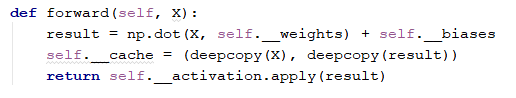
\includegraphics[width=14cm]{hidden_forward}  
		\caption{\label{fig:hidden_forward} Operația forward a clasei HiddenLayer}
	\end{figure}

	\newpage
	
	Stratul de tip Convolution va avea o perspectivă diferită asupra funcției follow:
	\begin{itemize}
		
	\item	 De data aceasta datele de intrare vin de forma unei matrici 4-dimensionale. Prima dimensiune este responsabila pentru stocarea datelor de intrare, reprezentate de data aceasta sub forma unei matrici 3-dimensioanle (o matrice cu multiple canale de valori ale pixelilor sau un feature-map).
	
	\item	Clasa va deține și va defini o matrice 3-dimensională, reprezentând filtrele de convoluție. Asemănător datelor de intrare, fiecare element din prima dimensiune a matricii este un filtru de forma unei matrici bi-dimensionale. În scopul ușurării procesării operațiilor de convoluție, despre care vom discuta în cele ce urmeaza, filtrele vor fi de forma 1X(n*n), unde n este o dimensiune a filtrului.
	
	
	\item	Pentru a realiza operația de convoluție am recurs la abordarea folosind funcțiile im2col, respectiv col2im. Scopul operației im2col, este de a rearanja structura matricii de intrare, astfel încât operația de convoluție sa fie redusă la o înmulțire de matrici.
	
	\item	Odată ce datele de intrare au fost procesate și remodelate de către funcția im2col, vom realiza o înmulțire de matrici cu datele remodelate și filtrele stratului. După aplicarea operației de col2im pentru restabilirea formei inițiale, vom obține rezultatul convoluției filtrelor asurpa datelor de intrare.
	
	
	\item	Dorim ca operația de convoluție să nu reducă dimensiunea datelor de intrare. Pentru respectarea acestei constrângeri, atributului zeroPadding, al clasei ConvLayer, ii va fi setat, odată cu inițializarea obiectului, o valoare care reprezintă numărul de coloane și randuri de valori de 0 ce trebuiesc adăugate datelor de intrare pentru a-și păstra forma după operația de convoluție.
	
	\item	După finalizarea operației de convoluție, vom readuce rezultatul în forma inițială utilizând funcția col2im, vom aplica funcția de activare și vom returna valoarea.(Vezi Fig. \ref{fig:conv_forward})

	\end{itemize}

	\vfill
	
	\begin{figure}[H]
		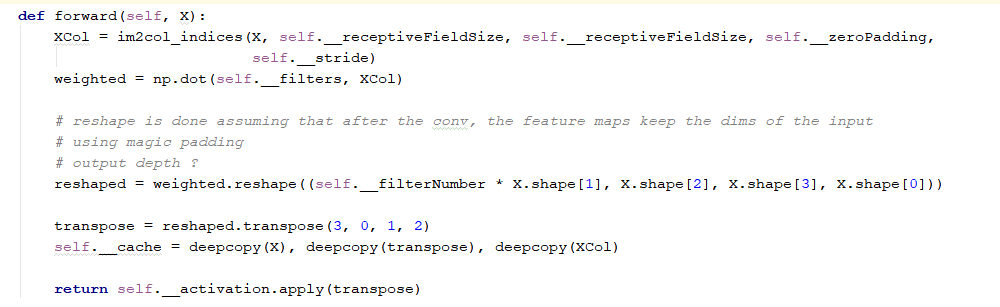
\includegraphics[width=14cm]{conv_forward}  
		\caption{\label{fig:conv_forward} Operația forward a clasei ConvLayer}
	\end{figure}

	
	Stratul de tip Pooling, deși asemănător stratului de tip Convolution, definește follow astfel:
	
	\begin{itemize}
	\item	Datele de intrare vor avea aceeasi forma ca și stratul de tip Convolution. 
	
	\item	Vom reutiliza funcția im2col datorită operației de Max Pooling, care este o operație asemănătoare convoluției. Aplicând funcția argmax, a bibliotecii NumPy, pe rezultatul funcției im2col, vom obține poziția fiecărui element cu valoare maximă de pe fiecare coloană, i.e rezultatul maxim în interiorul fiecărui porțiuni posibile operației de convoluție. 
	
	\item	Odată ce avem pozițiile fiecărui element maxim, vom crea, pentru fiecare dată de intrare, o matrice nouă care conține doar elementele cu valoarea maximă. Rezultatul obținut reprezintă o versiune cu o dimensiune redusă față de cea inițială și cu detalii mai pronunțate. La finalul procesării returnăm rezultatul.	(Vezi Fig. \ref{fig:pool_forward})
	\end{itemize}

	\vfill
	
	\begin{figure}[H]
		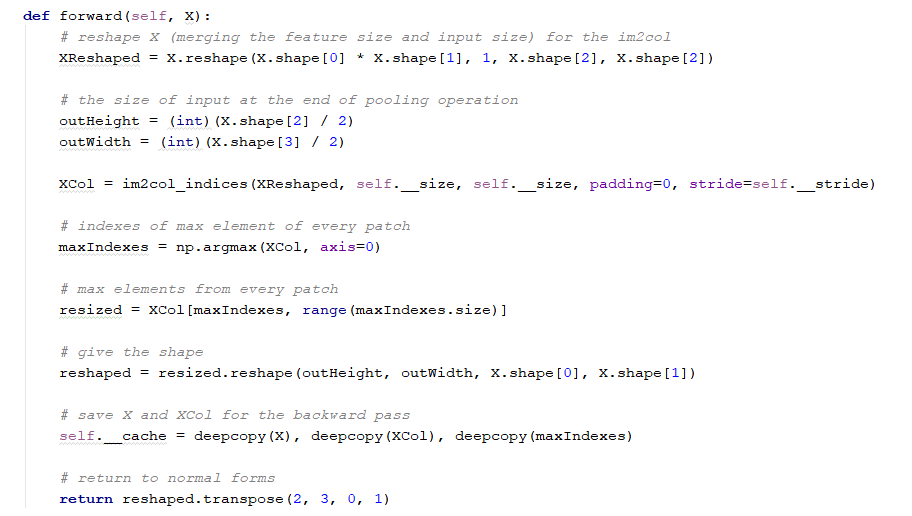
\includegraphics[width=15cm, height=7cm]{pool_forward}  
		\caption{\label{fig:pool_forward} Operația forward a clasei PoolingLayer}
	\end{figure}
	
	
	În scopul rezolvării incompatibilității între cele doua tipuri de straturi, Convolution și Hidden, la nivelul datelor de intrare si iesire, introducem un tip de strat a cărui funcție forward, este responsabil de conversia între cele doua reprezentări.
	 
	Pentru a realiza conversia, am folosit metoda reshape a componentelor de tip numpy.ndarray. (Vezi Fig. \ref{fig:reshape})
	
	\begin{figure}[H]
		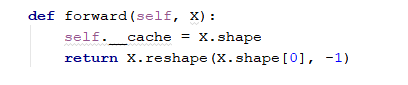
\includegraphics[width=10cm]{reshape}  
		\caption{\label{fig:reshape} Operația forward a clasei FlatteningLayer}
	\end{figure}
	
	În momentul în care datele de intrare au finalizat un circuit prin lanțul de straturi configurat, iar mutațiile au fost aplicate, este momentul să folosim un clasificator pentru a obține o decizie. 
	
	Aplicația definește un singur tip de clasificator, în scopul contextului problemei noastre, dar permite adăugarea sau implementarea mai multor tipuri de clasificatoare pe aceeași idee, a conceptului de polimorfism. 
	
	Ultimului strat adăugat în configurație, îi revine datoria de a reduce dimensiunea de ieșire dupa procesare, la numărul de clase ce trebuiesc clasificate. Acest lucru în cazul nostru este realizat de un strat de tip Hidden care are n ca dimensiune de intrare si k dimensiune de ieșire (unde n este dimensiunea datelor de ieșire al stratului precedent iar k este numărul total de clase ce trebuiesc clasificate).
	 
	Implementarea funcției Softmax de clasificare se face în clasa Softmax din pachetul model. Algoritmul folosește functia exponent al bibliotecii NumPy pentru a reprezenta valorile obținute sub forma de probabilități, iar mai apoi le normalizează. (Vezi Fig. \ref{fig:softmax})
	
	\vfill
	
	\begin{figure}[H]
		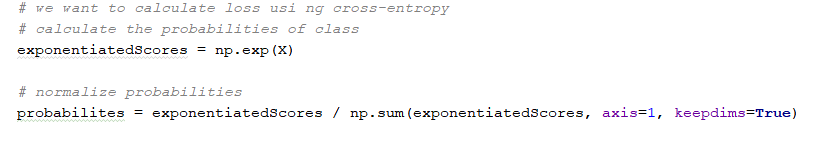
\includegraphics[width=10cm]{softmax}
		\caption{\label{fig:softmax} Cod sursă pentru algoritmul Softmax}
	\end{figure}

	\newpage
	
	După finalizarea acestor pasi, vom obține pentru fiecare intrare un vector de dimensiune k care conține probabilitatea pentru fiecare clasă pe poziția i ( 0 >= i > k, unde k este numărul de clase). Datorită faptului că avem doar o singură clasă corectă, corespunzătoare fiecărei date de intrare, cunoscută în momentul antrenării, dorim să aflăm cum a influențat modelul nostru decizia și cum putem sa îl penalizăm, în cazul unei decizii eronate. Pentru a realiza acest lucru, vom calcula funcția de eroare cross-entropy (Vezi Fig. \ref{fig:cross-entropy}). Avantajul utilizării acestei funcții de eroare, este valoarea sa descrecătoare exponențial, pe măsură ce x creste. (Vezi Fig. \ref{fig:logloss})
	
	\begin{figure}[H]
		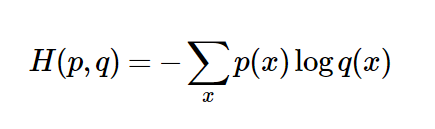
\includegraphics[width=10cm]{cross-entropy}
		\caption{\label{fig:cross-entropy} Funcția cross-entropy, unde p este un vector cu clasele corecte iar q este un vector cu predicțiile modelului}
	\end{figure}	
	
	\vfill
	
	\begin{figure}[H]
		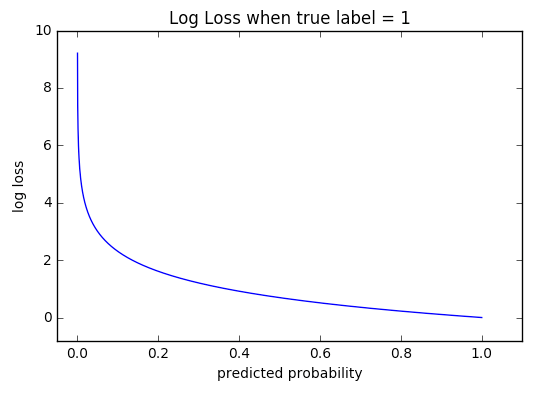
\includegraphics[width=10cm]{logloss}
		\caption{\label{fig:logloss} Reprezentare grafică a funcției de eroare logaritm}
	\end{figure}


	Scopul final al utilizării acestei funcții de eroare, este de a obține valorile de penalizare ce trebuiesc aplicate ponderilor ce au influențat această decizie. (vezi Fig. \ref{fig:error})
	
	\begin{figure}[H]
		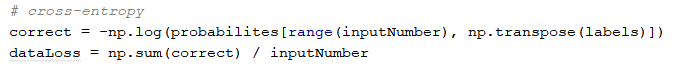
\includegraphics[width=14cm]{error}
		\caption{\label{fig:error} Calcularea erorii prin funcția logaritm}
	\end{figure}

	
	Implicit, clasificatorul Softmax va calcula funcția de regularizare L2, utilizând parametrul configurat, regularization, asupra ponderilor straturilor configurate. Funcția L2 ne va da o valoare reprezentând eroarea de regularizare, care va urma a fi adaugată la eroarea funcției logaritm în scopul evitării situației de overfitting. (vezi Fig. \ref{l2})


	\begin{figure}[H]
		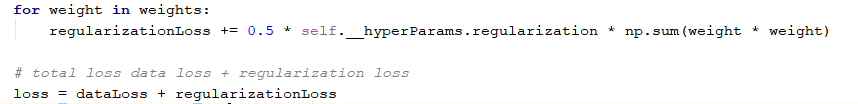
\includegraphics[width=15cm]{l2}
		\caption{\label{fig:l2} Calcularea regularizării L2 și eroarea totală}
	\end{figure}

	Dupa ce clasificatorul va returna valorile de erori corespunzătoare fiecărei intrări, se va finaliza etapa de feed-forward și jumătate din circuitul de antrenare al modelului. Următorul pas va fi de a regla ponderile țn funcție de această eroare, prin etapa de back-propagation.
	 
	Asemănător etapei de inferență, propagarea erorii se realizează diferit de la un tip de strat la altul. De aceea aplicația noastră declara o metodă abstractă backprop, implementată de către fiecare tip de layer.
	
	Propagarea erorii se realizează prin regula derivării în lanț, regulă a derivatelor compuse care spune ca dacă o variabilă z depinde o variabilă y, care la rândul ei depinde de o variabilă x, atunci z depinde și de x și se numesc variabile dependente, de unde rezultă formula:  dz/dx  =dz/dy*dy/dx
	
	Astfel aplicând regula lanțului derivatelor în contextul nostru, fiecare strat își va calcula derivata în funcție de derivata stratului următor. În cazul ultimului strat, cel ce precede clasificatorul, derivata va fi chiar rezultatul funcției de eroare.
	
	\vfill
	Operatia backprop a stratului de tip Hidden se produce astfel:
	\begin{itemize}
	\item	Vom calcula derivata funcției de activare. Această derivată va fi implementată de către clasele de tip Activation.
	
	\item	Derivata funcției de activare va fi multplicată (operația np.dot, a bibliotecii NumPy) cu datele de intrare procesate inițial (acestea sunt salvate în memorie la momentul etapei de feed-forward).
	
	
	\item	Se calculează noile derivate ale ponderilor, utilizând aceași operație de multiplicare. Odată ce obținem derivatele ponderilor, putem modifica ponderile. Putem profita de faptul că derivatele indică panta funcției, pentru a modifica ponderile în scopul convergerii. Utilizând parametrul din etapa de configurație, stepSize (parametru ce influențează viteza de convergere), vom modifica ponderile astfel încât la următorul pas de feed-forward acestea vor avea o eroare diminuată asupra aceluiasi set de intrări.
	
	\item	Odata ce ponderile au fost modificate, vom repeta pasul derivării pentru datele de intrare si noile ponderi. (Vezi Fig. \ref{fig:hidden_backprop})\newline
	\end{itemize}	

	\begin{figure}[H]
	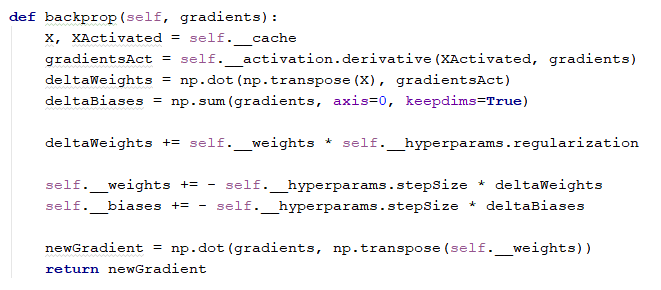
\includegraphics[width=15cm]{hidden_backprop}
	\caption{\label{fig:hidden_backprop} Operația backprop a stratului Hidden}
	\end{figure}



	Operația backprop a stratului de tip Convolution:
	\begin{itemize}
	\item	Conceptul propagării este asemănător celui de tip Hidden. Diferența va fi facută la modul în care datele și derivatele sunt reprezentate. Vom reutiliza operația col2im pentru a readuce datele în starea inițială după proceserea acestora.
	La finalul etapei de propagare a stratului de tip Convolution, filtrele vor avea modificările aduse de către funcția de eroare. (Vezi Fig. \ref{fig:conv_backprop})
	\end{itemize}

	\begin{figure}[H]
	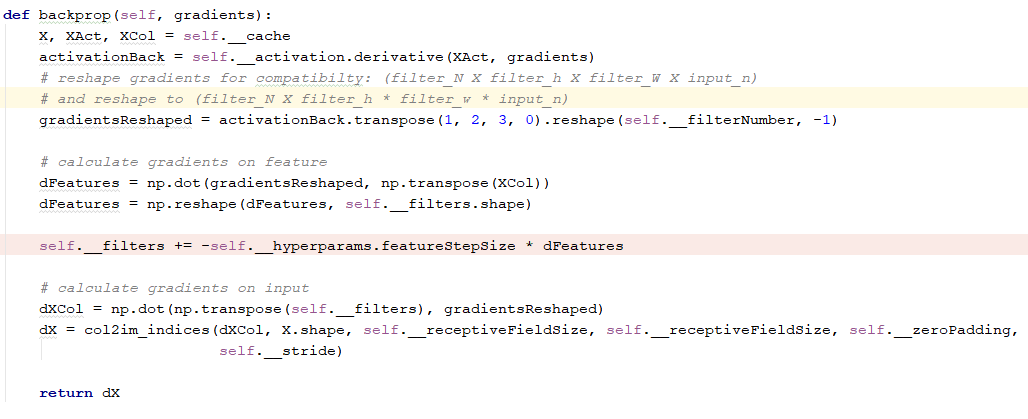
\includegraphics[width=17cm]{conv_back}
	\caption{\label{fig:conv_backprop} Operația backprop a stratului de Convolution}
	\end{figure}
	


	Configurarea arhitecturii a fost concepută să urmărească un sablon cât mai simplu. Definirea arhitecturii și a parametrilor de antrenare va fi realizată prin crearea unui fișier de tip JSON. 
	Acest fișier va fi plasat în folderul requests din structura proiectului.La pornirea aplicației, utilizatorul va putea selecta numele fișierului ce se dorește a reprezenta arhitectura. (Vezi Fig. \ref{fig:config_json}) 
	
	\begin{figure}[H]
		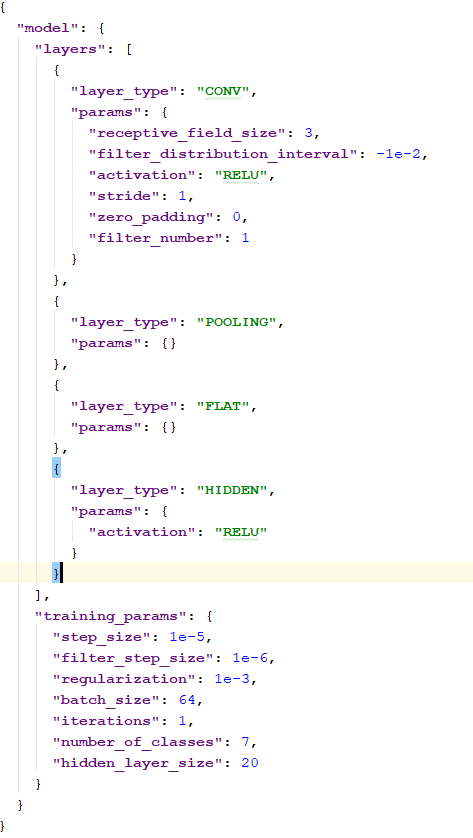
\includegraphics[width=10cm]{json_config}
		\caption{\label{fig:config_json} Fișier de configurare JSON}
	\end{figure}
	
	Aplicația va conține o structură ierarhică unde iși va gestiona resursele. Aceste resurse pot fi găsite în directorul resources. (Vezi Fig. \ref{fig:resources-folder})
	
	Pentru a asigura integritatea platformei, aplicația va verifica existența structurii de directoare ce conțin configurări (requests) și date de antrenare(dataset). Dacă aceste constrângeri lipsesc, utilizatorul va fi avertizat printr-un mesaj de eroare. Restul structurilor vor fi generate la momentul rulării primei rutine de antrenare.
	
	Structura de resurse este după cum urmează:
	\begin{itemize}
	\item Folderul dataset va conține o structură de forma processed/{k} unde n este k este un număr între 0 și n este numărul de clase.
	
	\item Folderul requests va conține configurările în format JSON.
	
	\item Folderul features va conține imagini rezultate pe urma operațiilor de convoluție a straturilor și au un scop analitic.
	
	\item Folderul history va conține, la finalul etapei de antrenare, un fișier de tip HTML ce va conține structura modelului antrenat (JSON) si un tabel cu progresul predicției la fiecare epocă.
	
	\item Folder model-data va conține modelul antrenat în format JSON. Acest fișier va putea fi distribuit mai departe la finalul etapei de antrenare.
	
	\end{itemize}
	
	\begin{figure}[H]
		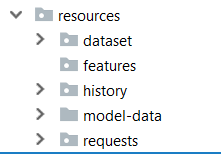
\includegraphics[width=7cm]{resources-folder}
		\caption{\label{fig:resources-folder} Structura resurselor}
	\end{figure}

	
	Pe baza configurării JSON, definirea straturilor și crearea lor va fi realizată prin metoda addLayer a clasei LayersBuilder. Metoda primește un parametru ce reprezintă tipul de strat ce se doreste a fi creat și un obiect ce reprezintă parametrii necesari construirii tipului respectiv de strat. Scopul clasei LayersBuilder este de a ușura crearea arhitecturii modelului prin izolarea logicii de construire si concatenarea tipurilor de straturi. (vezi Fig. \ref{fig:add_layers})	
	
	\begin{figure}[H]
		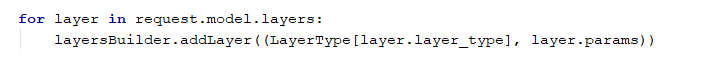
\includegraphics[width=17cm]{add_layers}
		\caption{\label{fig:add_layers} Adaugarea straturilor}
	\end{figure}

	Logica din spate a clasei LayerBuilder se ocupă de ordinea în care straturile sunt adăugate, de compatibilitățile dintre straturi, de respectarea unor constrângeri și de validare.
	
	Primul pas în construirea straturilor este de a aduna informații despre structura straturilor, cum ar fi adâncimea totală pe care o vom aveam, datorată straturilor de convoluție și a filtrelor,  numărul de reduceri de dimensiune pe care le vom aplica prin straturile de tip Pooling și numărul de straturi de tipuri Hidden. Acestea sunt necesare pentru construirea modelului, dat fiind faptul că straturile vor avea o dependență strânsă între ele.  (vezi Fig. \ref{fig:layer_builder})
	
	\begin{figure}[H]
		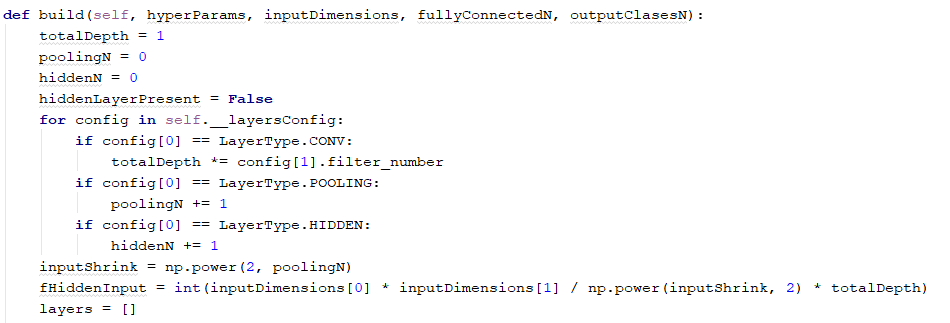
\includegraphics[width=17cm]{layer_builder}
		\caption{\label{fig:layer_builder} Pregătirea datelor; metoda build}
	\end{figure}
	

	După ce au fost adunate destule informații generale legate de structura modelului, vom începe etapa de construcție a modelului, prin crearea unei liste de obiecte de tip Layer. Parametrii de regularizare și funcția de activare vor fi transmise ca și parametri la momentul inițializării tipului de strat. Dupa ce lista a fost construită cu succes,  va fi returnată spre a fi folosită de obiectul de tip Model. (Vezi Fig. \ref{fig:actual_build})
	
	
	\begin{figure}[H]
		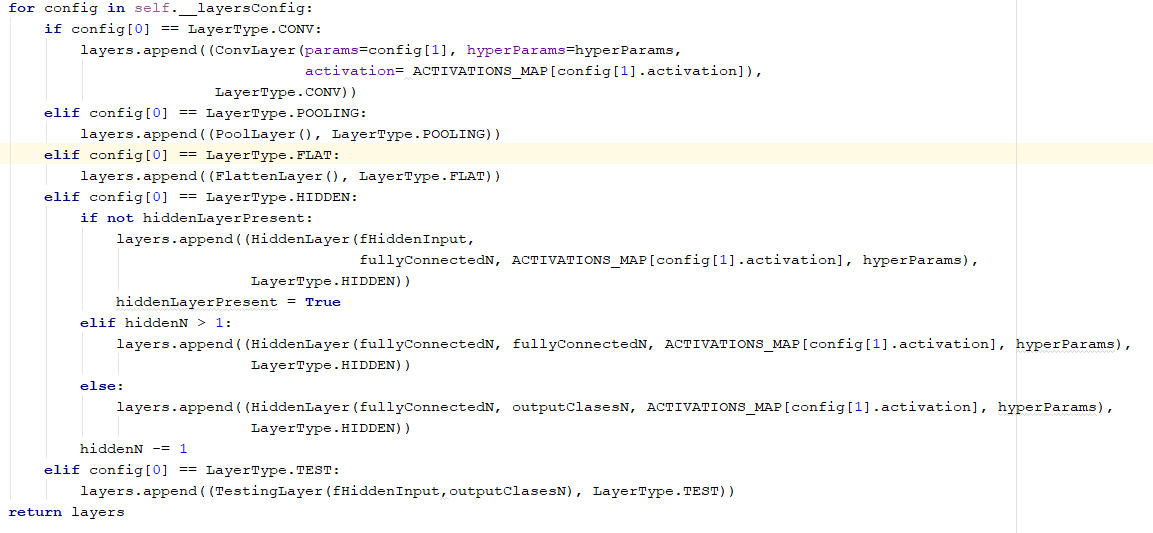
\includegraphics[width=17cm]{actual_build}
		\caption{\label{fig:actual_build} Construcția listei de straturi}
	\end{figure}


	După ce avem lista de straturi consistent configurată, vom crea un obiect de tip Model, entitatea care va modela parametrii. (vezi Fig \ref{fig:train})
	
	\begin{figure}[H]
		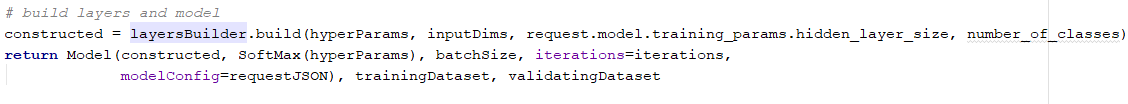
\includegraphics[width=17cm]{train}
		\caption{\label{fig:train} Crearea modelului și antrenarea sa}
	\end{figure}
	
	\newpage
	\subsection{Modulul de inferență și aplicația client Android}
	
	Pentru a putea utiliza într-un mod practic un model antrenat, am implementat o aplicație Android ce folosește imagini primite ca și stream de la cameră în scopul procesării acestora utilizând un model primit prin protocolul HTTP peste TCP/IP de la un server ce găzduiește modele antrenate. 
	Aplicația folosește un modul Java a cărui scop este separarea logicii de configurare a operațiilor de inferență, de scopul business al aplicației. \newline
	
	Datorită limbajului de programare Java și a structurii modulare, biblioteca pentru inferență poate fi utilizată și de alte platforme și sisteme operare.
	
	Utilizarea bibliotecii de configurare și inferență va fi folosită sub forma de dependență Gradle. Pentru a putea expune dependețele ca și repository compatibil cu Gradle am utilizat serviciile oferite www.jitpack.io și www.github.com. 
	
	Prin separarea acestor module, putem beneficia și de avantajul versionării oferite de serviciului git. Astfel modificările aduse în paralel asupra aplicației, respectiv bilbiotecii de inferență, vor fi gestionate mai usor.
	
	Scopul modulului de inferență este de a reconstitui un model de rețele neuronale convoluționale pe baza unui model de configurații oferit de către platforma Python de antrenare, discutată în capitolul anterior. Separarea logicii este facută astfel încât logica de transfer al modelului antrenat să fie exclusă din implementarea inferenței. Aplicația client se va ocupa de preluarea modelului antrenat de pe un server, transportat în format JSON, după care va construi modelul de inferență pe baza parsării modelului JSON. (Vezi Fig. \ref{fig:model-json})
	
	\vfill
	
	\begin{figure}[H]
		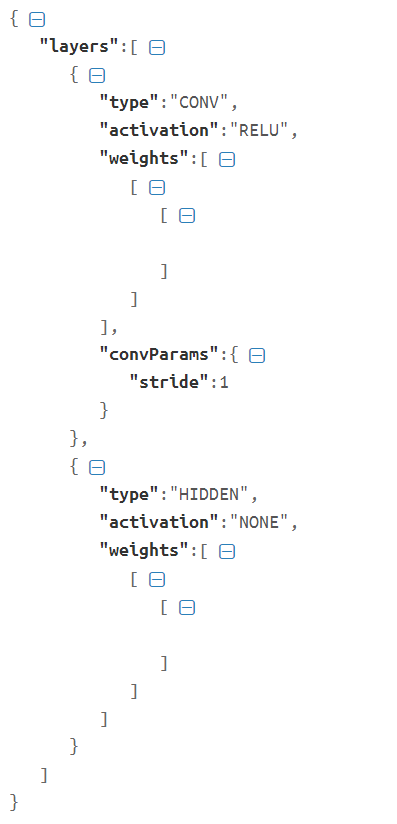
\includegraphics[width=10cm]{model-json}
		\caption{\label{fig:model-json} Exemplu de reprezentare a modelului in format JSON}
	\end{figure}

	\newpage
	
	Modulul este bazat pe operații matematice pentru a realiza inferența modelului. Arhitectura modulului este realizată într-o maniera corespunzătoare paradigmei OOP, în scopul usurării operațiilor și a genericității lor. Astfel obtinem 3 entități de baza, pe baza cărora se va dezvolta logica de inferența.Interfetele SimpleLayer, ComplexLayer si TransitionLayer definesc metoda forward a fiecărui tip de layer dintr-o rețea neuronală.(Vezi Fig. \ref{fig:layers-architecture})
	
	
	\begin{figure}[H]
		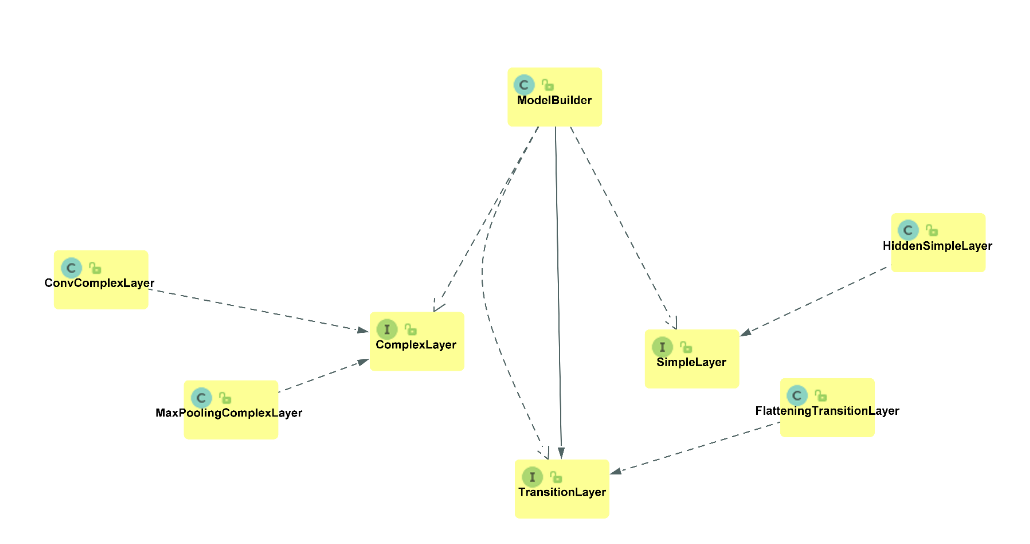
\includegraphics[width=15cm]{cnn-inference-class-graph}
		\caption{\label{fig:layers-architecture} Diagrama de clase a entităților de bază din modulul de inferență}
	\end{figure}

	Implementarea entităților de bază este realizată de tipurile concrete de straturi, și anume: HiddenSimpleLayer, ConvComplexLayer, MaxPoolingComplexLayer și FlatteningTransitionLayer. Pentru a urmări dezvoltarea unui cod sugestiv am urmărit convenția de denumire a straturile în felul următor: numele tipului de strat, urmat de complexitatea stratului (Simple sau Complex).
	
	Scopul stratului de tip TransitionLayer este de a crea o compatibilitate între datele de ieșire ale stratului de tip ComplexLayer și datele de intrare ale tipului SimpleLayer. 
	
	O implementare a stratului SimpleLayer, în contextul actual, este realizată de clasa HiddenSimpleLayer. Aceasta reprezintă tipul de strat ascuns din componența unui model de rețele neuronale. Aceasta deține câmpuri necesare operației de mutație: ponderile (weights), biases și funcția de activare. (Vezi Fig. \ref{fig:simple-layer})
	
	
	\begin{figure}[H]
		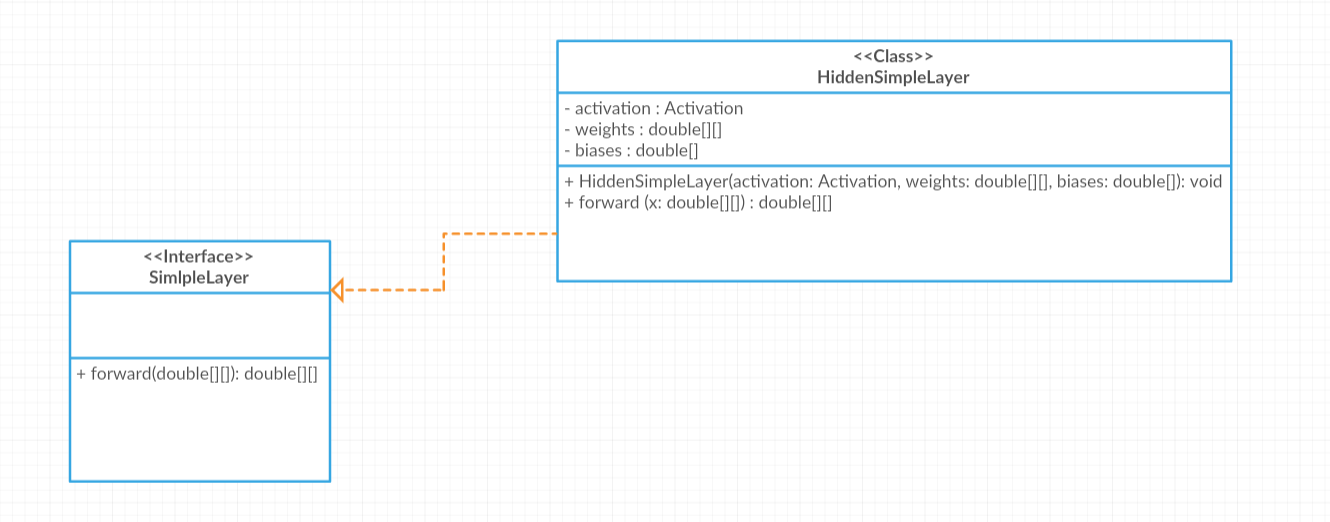
\includegraphics[width=15cm]{simple-layer}
		\caption{\label{fig:simple-layer} O implementare a interfeței SimpleLayer; HiddenSimpleLayer}
	\end{figure}

	\vfill


	Interfața ComplexLayer se regăsește în două tipuri de straturi prezente în modul, și anume: ConvComplexLayer și MaxPoolingComplexLayer. (Vezi Fig. \ref{fig:complex-layer})
	
		\begin{figure}[H]
		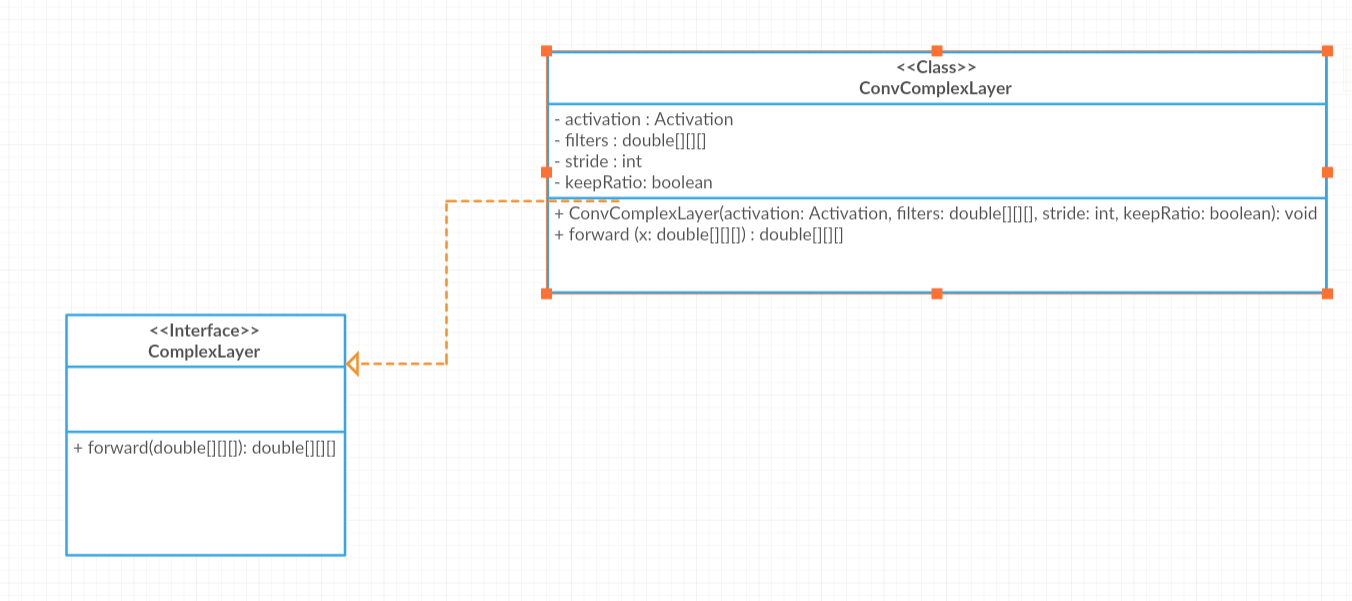
\includegraphics[width=15cm]{conv-complex-layer}
		\caption{\label{fig:complex-layer} O implementare a interfeței ComplexLayer. ConvComplexLayer}
	\end{figure}

	Prin utilizarea interfețelor putem generaliza operațiile și tipurile de straturi. Astfel inferența se reduce la o listă de obiecte SimpleLayer, o listă de obiecte ComplexLayer și un element tranzient de tip Transition.
	
	In urma finalizării pasului de inferență, se va returna un obiect de tipul PredictionResult. Acest obiect va avea in componență atât rezultatul ne-normalizat al procesului de inferență cât și probabilitățile pentru fiecare clasa.(Vezi Fig. \ref{fig:prediction-result})
	
	\begin{figure}[H]
		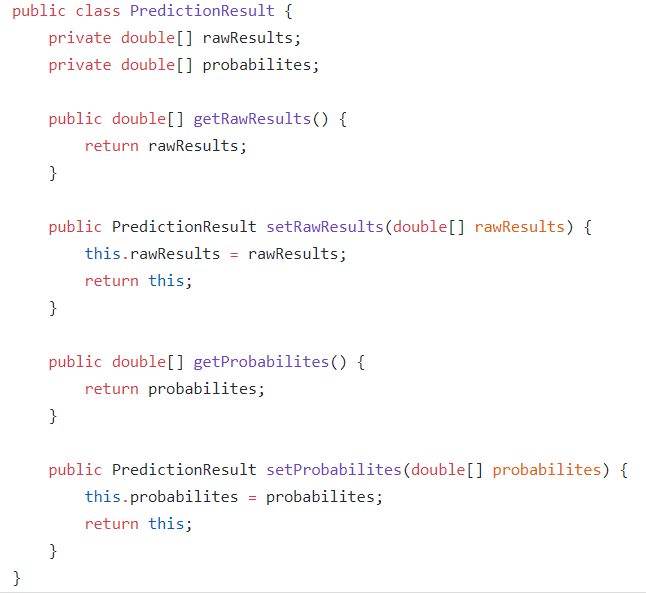
\includegraphics[width=15cm]{prediction-result}
		\caption{\label{fig:prediction-result} Componența clasei PredictionResult}
	\end{figure}
	
	\vfill
	
	Aplicația Android iși va actualiza modelul predictiv printr-un call http la un server (în cazul nostru, serverul fiind un mock doar de expunere a modelului json), și va reactualiza componența modulului de inferență. Pentru a putea crea un obiect Model al bibliotecii de inferență, vom utiliza clasa NetworkModelBuilder. Aceasta va fi interfața client ce va sta între operațiile de inferență și interfața vizuală a utilizatorului. Clasa NetworkModelBuilder definește o metodă build, ce primește un obiect de tip ModelDescriptor și unul de tip Configuration și returnează un obiect de tipul NetworkModel ce va putea fi utilizat în stratul de View. 
	
	\newpage
	
	După finalizarea configurării modelului, se va incepe un proces de stream al imaginilor. Acest stream va fi utilizat atât pentru crearea unei previzualizări dar și pentru procesare. Fiecare cadru va fi pregătit pentru procesare (reducere în dimensiune și centrare) și va fi trimis sub format Bitmap obiectului de tip NetworkModel. 
	Acesta va extrage valoriile reale corespunzătoare obiectului de tip Bitmap și le va trimite spre a fi procesate de modulul de inferență. După finalizarea unui ciclu de predicție, obiectul de tip NetworkModel va returna o predicție, pe baza căreia activitatea iși va actualiza elementele.
	(Vezi Fig. \ref{fig:prediction-sequence})\newline
	
	\begin{figure}[H]
		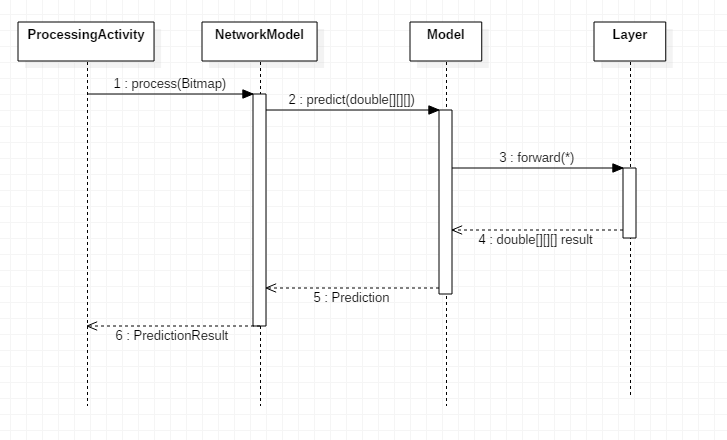
\includegraphics[width=15cm]{sequence}
		\caption{\label{fig:prediction-sequence} Diagrama de secvență a funcționalității de procesare}
	\end{figure}

	\newpage
	Aplicația va afișa un preview al camerei iar in stânga va afișa predicțiile pentru fiecare cadru. Deasupra predicțiilor va fi afișat timpul de procesare în milisecunde.
	
	(Vezi Fig. \ref{fig:mobile-app})\newline 	
	
	
		\begin{figure}[H]
		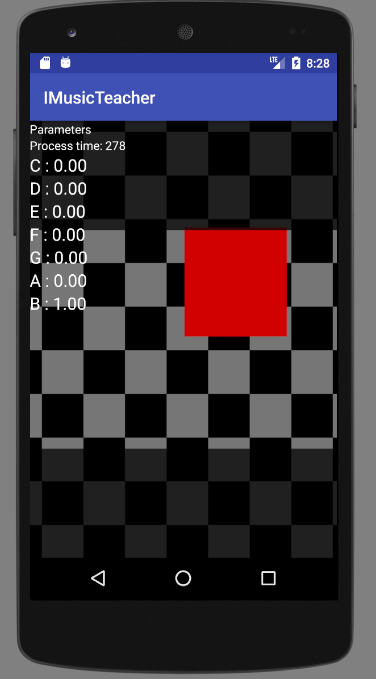
\includegraphics[width=10cm]{mobile-app}
		\caption{\label{fig:mobile-app} Ecranul principal al aplicației}
	\end{figure}
\end{document}